% Created 2022-07-27 水 14:50
% Intended LaTeX compiler: pdflatex
\documentclass[11pt]{scrartcl}
                   \usepackage[utf8]{inputenc}
                   \usepackage{cmbright}
                   \usepackage[usenames,dvipsnames]{xcolor}
                   \usepackage{graphicx,longtable,url,rotating}
                   \usepackage{amsmath}
                   \usepackage{amsfonts}
                   \usepackage{amssymb}
                   \usepackage{subfig}
                   \usepackage{minted}
                   \usepackage{algpseudocode}
                   \usepackage[round]{natbib}
                   \usepackage{alltt}
                   \renewenvironment{verbatim}{\begin{alltt} \scriptsize \color{Bittersweet} \vspace{0.2cm} }{\vspace{0.2cm} \end{alltt} v\normalsize \color{black}}
\definecolor{lightcolor}{gray}{.55}
\definecolor{shadecolor}{gray}{.95}
\usepackage{minted}
\usepackage{multicol}

                   \usepackage{hyperref}
                   \hypersetup{colorlinks=true,pagebackref=true,urlcolor=orange}
\author{Nilton Liuji Kamiji, Christophe Pouzat, Aline Duarte, Antonio Roque, \\Antonio Galves}
\date{\today}
\title{Implementaion of the Potjans Diesmann microcircuit model using the classical Galves-L\"{o}cherbach neuron model}
\hypersetup{
 pdfauthor={Nilton Liuji Kamiji, Christophe Pouzat, Aline Duarte, Antonio Roque, \\Antonio Galves},
 pdftitle={Implementaion of the Potjans Diesmann microcircuit model using the classical Galves-L\"{o}cherbach neuron model},
 pdfkeywords={},
 pdfsubject={},
 pdfcreator={Emacs 27.2 (Org mode 9.4.4)}, 
 pdflang={English}}
\begin{document}

\maketitle
\tableofcontents
\pagebreak
\listoffigures
\pagebreak

\section{Introduction}
\label{sec:orgf8c6b86}

Implementation of the Potjans and Diesmann \cite{PotjansDiesmann2014} microcircuit model using the classical Galves-L\"{o}cherbach neuron model \cite{GalvesLocherbach2013} in discrete time.

\section{Model definition}
\label{sec:org5936f3e}

\subsection{The original PD model}
\label{sec:org78807a2}
\label{orga6c4122}

The PD model (Potjans and Diesmann, 2014) consists of 8 neuronal populations, representing excitatory and inhibitory populations of 4 cortical layers, namely, layers 2/3 (L23e/i), 4 (L4e/i), 5 (L5e/i) and 6 (L6e/i), where e denotes excitatory and i inhibitory. The number of neurons of each population is shown in table \ref{table:PD_num_neurons}, which totalizes 77169 neurons.
\begin{table}[htbp]
    \centering
    \caption{Number of neurons per cortical layer}
    \label{table:PD_num_neurons}
    \begin{tabular}{llllllll}
         \multicolumn{1}{c}{L23e} & \multicolumn{1}{c}{L23i} & \multicolumn{1}{c}{L4e} & \multicolumn{1}{c}{L4i} & \multicolumn{1}{c}{L5e} & \multicolumn{1}{c}{L5i} & \multicolumn{1}{c}{L6e} & \multicolumn{1}{c}{L6i} \\
         20683 & 5834 & 21915 & 5479 & 4850 & 1065 & 14395 & 2948 
    \end{tabular}
\end{table}

\subsubsection{Membrane potential dynamics}
\label{sec:org9c6a170}
\label{orga332c11}

All neurons are described with the same LIF (leaky integrate-and-fire) dynamics (eq. (\ref{eq:LIF}))
\begin{equation}
  \begin{aligned}
    \frac{dV_m(t)}{dt} &= \begin{cases} 0 & \text{if neuron is refractory} \\
    -\frac{V_m(t)}{\tau_m} + \frac{S_{syn}^i(t)}{C_m} & \text{otherwise}
    \end{cases} \\
    \frac{dI_{syn}(t)}{dt} &= \begin{cases} 0 & \text{if neuron is refractory} \\
    -\frac{I_{syn}(t)}{\tau_{syn}} + \sum_j{W_j} & \text{otherwise}
    \end{cases} \\
    \text{if } V_m^i(t) \geq V_{th} &\quad \text{neuron spiked and refractory}
  \end{aligned}
  \label{eq:LIF}
\end{equation}
where \(V_m(t)\) is the membrane potential, \(\tau_m = 10\) ms is the membrane time constant representing the leakage effect, \(C_m = 250\) pF the membrane capacitance, \(V_{th} = 15\) mV the threshold potential in which a neuron fires when its membrane potential exceeds this value, \(I_{syn}(t)\) the membrane current elicited by synaptic inputs from pre-synaptic neurons  \(j\) (\(W_j\)), and \(\tau_{syn} = 0.5\) ms the synaptic time constant indicating the dynamics of synaptic receptor channel. The refractory period (\(\tau_{ref}\)), the period in which a neuron stays silent after emmiting a spike, was 2 ms.


\subsubsection{The graph of interaction}
\label{sec:org03c23f7}
\label{orgf7bab06}

Neurons are connected following the connection probability between neuronal populations shown in table \ref{table:PD_conectivity}.
The resulting graph of interaction is a directed graph with nearly 300 million edges.

\begin{table}[htbp]
    \centering
    \caption{\label{table:PD_conectivity} Connection probability between neuronal populations
    }
    \begin{tabular}{lccccccccc}
         &  & \multicolumn{8}{c}{from} \tabularnewline
         &  & L23e & L23i & L4e & L4i & L5e & L5i & L6e & L6i \tabularnewline
         & L23e & 0.101 & 0.169 & 0.044 & 0.082 & 0.032 & 0.0 & 0.008 & 0.0 \tabularnewline
         & L23i & 0.135 & 0.137 & 0.032 & 0.052 & 0.075 & 0.0 & 0.004 & 0.0 \tabularnewline
         & L4e & 0.008 & 0.006 & 0.050 & 0.135 & 0.007 & 0.0003 & 0.045 & 0.0 \tabularnewline
         to & L4i & 0.069 & 0.003 & 0.079 & 0.160 & 0.003 & 0.0 & 0.106 & 0.0 \tabularnewline
         & L5e & 0.100 & 0.062 & 0.051 & 0.006 & 0.083 & 0.373 & 0.020 & 0.0 \tabularnewline
         & L5i & 0.055 & 0.027 & 0.026 & 0.002 & 0.060 & 0.316 & 0.009 & 0.0 \tabularnewline
         & L6e & 0.016 & 0.007 & 0.021 & 0.017 & 0.057 & 0.020 & 0.040 & 0.225 \tabularnewline
         & L6i & 0.036 & 0.001 & 0.003 & 0.001 & 0.028 & 0.008 & 0.066 & 0.144 
         \tabularnewline
    \end{tabular}
\end{table}

Moreover, synaptic connections between neurons \(j\) and \(i\) are described by the synaptic weights (\(w_{j \to i}\)) and transmission delay (\(d_{j \to i}\)), drawn from a clipped normal distribution, and are different for excitatory and inhibitory synapses as shown in table \ref{table:PD_synaptic_weight_delay}. \(dt\) is the simulation time step, indicating that synapse transmission requires at least one time step.

\begin{table}[htb!]
    \centering
    \caption{Synaptic weight and delay. Synaptic weights are clipped at 0, and synaptic delays are clipped at simulation step ($d_t = 0.1$ ms)}
    \label{table:PD_synaptic_weight_delay}
    \begin{tabular}{lcl}
        %  \multicolumn{2}{c}{excitatory} \\
         &
         $w_e$ & $\mathcal{N}$($\mu = 87.8, \sigma = 8.8$) pA; $w_e > 0$ \\
         excitatory & $d_e$ & $\mathcal{N}$($\mu=1.5 , \sigma = 0.75$) ms; $d_e \geq dt$ \\
        %  \multicolumn{2}{c}{inhibitory}  \\
         &
         $w_i$ & $\mathcal{N}$($\mu = -351.2, \sigma = 35.1$) pA; $w_i < 0$ \\
         inhibitory & $d_i$ & $\mathcal{N}$($\mu=0.8 , \sigma = 0.4$) ms; $d_i \geq dt$
    \end{tabular}
\end{table}

\textbf{Remark 1} A synaptic weight of \(87.8\) pA will elicit a maximum membrane potential change of approximately \(0.15\) mV.

\textbf{Remark 2} The number of synapses (\(K\)) between any two populations are calculated from:
\begin{equation}
    K = \frac{\log(1 - C_a)}{\log(1-1/(N_{pre}N_{post}))},
    \label{eq:PD_K}
\end{equation}
where \(C_a\) is the connection probability taken from table \ref{table:PD_conectivity}, \(N_{pre}\) and \(N_{post}\) the number of neurons in the pre- and post-synaptic population, respectively, taken from table \ref{table:PD_num_neurons}. The \(K\) pairs are then randomly chosen, so that multiple synapses with different parameter values for any pair can occur. This phenomenon is know as multapses.

\textbf{Remark 3} The connection weight between neurons of L4e to L23e is doubled, that is, taken from a clipped normal distribution of \(\mathcal{N}\)(\(\mu = 175.6, \sigma = 17.6\)) pA

\subsubsection{Background input}
\label{sec:org17601e4}
\label{org111cc73}

The network is driven by a constant external input that can be described as Poissonian spike trains (\(rate = 8\) Hz) or constant current. The number of external inputs is layer dependent as shown in table \ref{table:PD_ext_num_neurons}.

\begin{table}[htbp]
    \centering
    \caption{Number of external inputs onto each cortical layer}
    \label{table:PD_ext_num_neurons}
    \begin{tabular}{llllllll}
         \multicolumn{1}{c}{L23e} & \multicolumn{1}{c}{L23i} & \multicolumn{1}{c}{L4e} & \multicolumn{1}{c}{L4i} & \multicolumn{1}{c}{L5e} & \multicolumn{1}{c}{L5i} & \multicolumn{1}{c}{L6e} & \multicolumn{1}{c}{L6i} \\
         1600 & 1500 & 2100 & 1900 & 2000 & 1900 & 2900 & 2100 
    \end{tabular}
\end{table}

\textbf{Remark 1} In the case of Poissonian spike trains input, every neuron on each layer receives independent Poissonian spike trains with \(rate = 8 \times n\), where \(n\) is the number of external inputs, which is the same as generating \(n\) Poissonian spike trains of \(8\) Hz and applying all of it to the neuron. Note that all input has fixed weight and delay values of \(87.8\) pA and \(1.5\) ms, respectively.

\subsection{The GL model}
\label{sec:org40cdc39}
\label{orgcc3006a}

\subsubsection{Membrane Potential Process}
\label{sec:orge9de777}

The the dynamics (\emph{membrane potential process} - \textbf{MPP}) of the neuron is described as:
\begin{equation}
V_t(i) = \sum_j{ W_{j\rightarrow i}\sum_{s=L_t^i}^{t-1}{ \exp\left({-\frac{t-s-1}{\tau_i}}\right)X_{s-d_{j\rightarrow i}+1}(j) } },
\label{eq:MPP_1}
\end{equation}
where:
\begin{description}
\item[{\(j\)}] The \emph{presynaptic neuron}.
\item[{\(i\)}] The \emph{postsynaptic neuron}.
\item[{\(W_{j\rightarrow i} \in \mathbb{R}\)}] The \emph{synaptic weight}, if \(w_{j\rightarrow i} < 0\) the synapse is \emph{inhibitory}, if \(w_{j\rightarrow i} >0\) it is \emph{exitatory}.
\item[{\(d_{j\rightarrow i} \in \mathbb{R}^+\)}] The \emph{synaptic delay}, this accounts for the \emph{propagation time} of the spike from the soma of neuron \(j\) to the the synaptic terminal on neuron \(i\), as well as the time for the presynaptic vesicles to fuse upon spike arrival, the transmitter to diffuse and bind to the postsynaptic receptors and the latter to open.
\item[{\(L_t^i\)}] The \emph{last spike time} of neuron \(i\) prior to time \(t\).
\item[{\(\tau_i\)}] The decay time constat of the leakage effect of the neuron.
\item[{\(X_t(i)\)}] The \emph{spike train} of neuron \(i\) taking value in \{0,1\}, if \(X_t(i)=1\) means neuron \(i\) fired at time \(t\).
\end{description}

Note that eq. (\ref{eq:MPP_1}) can be described as a Markovian system as:
\begin{equation}
\begin{aligned}
V_{t+1}(i) =&\; e^{-1/\tau_i} V_t(i) + \sum_j{ W_{j \to i} X_{s-d_{j \to i}+1}(j) } \\
X_{t+1}(i) =& 
\begin{cases}
1 & \; \text{if neuron spiked; set } $V_{t+1}(i) = 0$. \\
0 & \; \text{otherwise}
\end{cases}
\end{aligned}
\label{eq:MPP_exp_final}
\end{equation}

\subsubsection{The firing probability function \(\Phi(V_t(i))\)}
\label{sec:org07e1b70}

The firing probability function (\(\Phi(V_t(i))\)) was determined so that the firing rate of the neuron to constant current input (FI-curve) reproduces that of the LIF neuron of the original PD model.

We consider the following function for \(\Phi(V)\)

\begin{equation}
\Phi(V) = \begin{cases}
0 & \text{if $V \leq V_{rheo}$}\\
[\gamma(V-V_{rheo})]^r & \text{if $V_{rheo} < V < V_{sat}$} \\
1 & \text{if $V \geq V_{sat} = V_{rheo} + 1/\gamma$}
\end{cases}
\label{eq:phi_full}
\end{equation}


Fig. \ref{fig:FI_curve} represents the FI-curve of the original LIF neuron (red) and that of the GL model (blue). The FI-curve for the GL neuron was obtained with \(\gamma=0.1 \text{ mV}^{-1}\) (i.e. there is a window of 10 mV for \(0 < \Phi(V) < 1\)), \(r=0.4\) and \(V_{rheo}=15\) mV (\color{red}-50 mV in Fig. \ref{fig:GL_Phi}; will be corrected in future version\color{black}), which is represented in Fig. \ref{fig:GL_Phi}.

\begin{multicols}{2}
  \begin{center}
    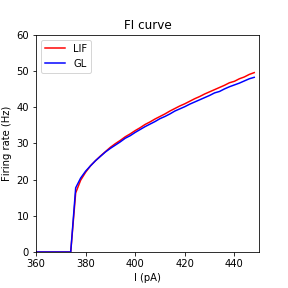
\includegraphics[width=\linewidth]{figures/FI_curve}
    \captionsetup{width=\linewidth}
    \captionof{figure}{FI curve of LIF (red) and GL (blue) neuron model.}
    \label{fig:FI_curve}
  \end{center}
  \begin{center}
    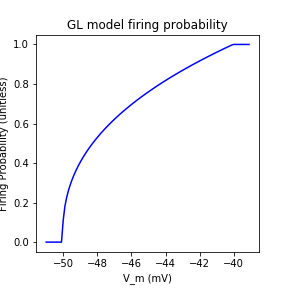
\includegraphics[width=\linewidth]{figures/GL_Phi}
    \captionsetup{width=\linewidth}
    \captionof{figure}{Firing rate ($\Phi(V)$) of the GL model.}
    \label{fig:GL_Phi}
  \end{center}
\end{multicols}


In practice a sequence of Bernoulli random variable is used at each time step: \(\{U_t(i)\}_{i \in I}\), \(U_t(i) \stackrel{IID}{\sim} \mathcal{B}\) and the \(X_{t+1}(i)\) are given by:
\begin{equation}\label{eq:X-evolution}
X_{t+1}(i) = \begin{cases}1 & \text{if } U_t(i) \le \phi_i\left(V_t(i)\right) \\ 0 & \text{otherwise}   \end{cases}
\end{equation}

\section{\texttt{C++} implementation}
\label{sec:orgd65e4e2}
TODO: write about the code

\subsection{Compile}
\label{sec:orgbcdc8ed}

\begin{minted}[bgcolor=shadecolor,fontsize=\scriptsize]{sh}
unzip dGLPD_delta.zip
mkdir bin
cd bin
cmake ../src
make
\end{minted}

\subsection{Execution time}
\label{sec:org6b2f41c}

Execution time was measured using time command. I have also measured simulation time of the original NEST implementation, however, only NEST 2.16.0, which was released on 2018-08-21, allowed to execute using a single process. All other NEST versions has restriction on the number of connections per virtual-process, requiring at least 3 virtual processes to simulate the PD model in full scale. When using a single process, our code was much faster than NEST 2.16.0. On the other hand, NEST 2.20.1 had a great improvement when using 4 virtual processes (OpenMP) when compared to NEST 2.16.0. However, if we compare user time, our code is comparable to that of NEST 2.20.1, suggesting that if similar approach is used to paralelize the code, we may obtain even better performance.

\subsubsection{Simulation time step of 1.0 ms}
\label{sec:org82adef5}

\begin{minted}[bgcolor=shadecolor,fontsize=\scriptsize]{sh}
time ./dGLPD_delta 11111 1000 1.0
\end{minted}

\begin{minted}[bgcolor=shadecolor,fontsize=\scriptsize]{text}
Random Number Generator Engine: xoroshiro128+
seed: 11111, Simulation time: 1000 ms, Simulation time step: 1 ms
prepare: 372.762 s
simulate(1000): 155.432 s

real    8m49.235s
user    8m26.601s
sys     0m21.554s
\end{minted}

\begin{figure}[htbp]
\centering
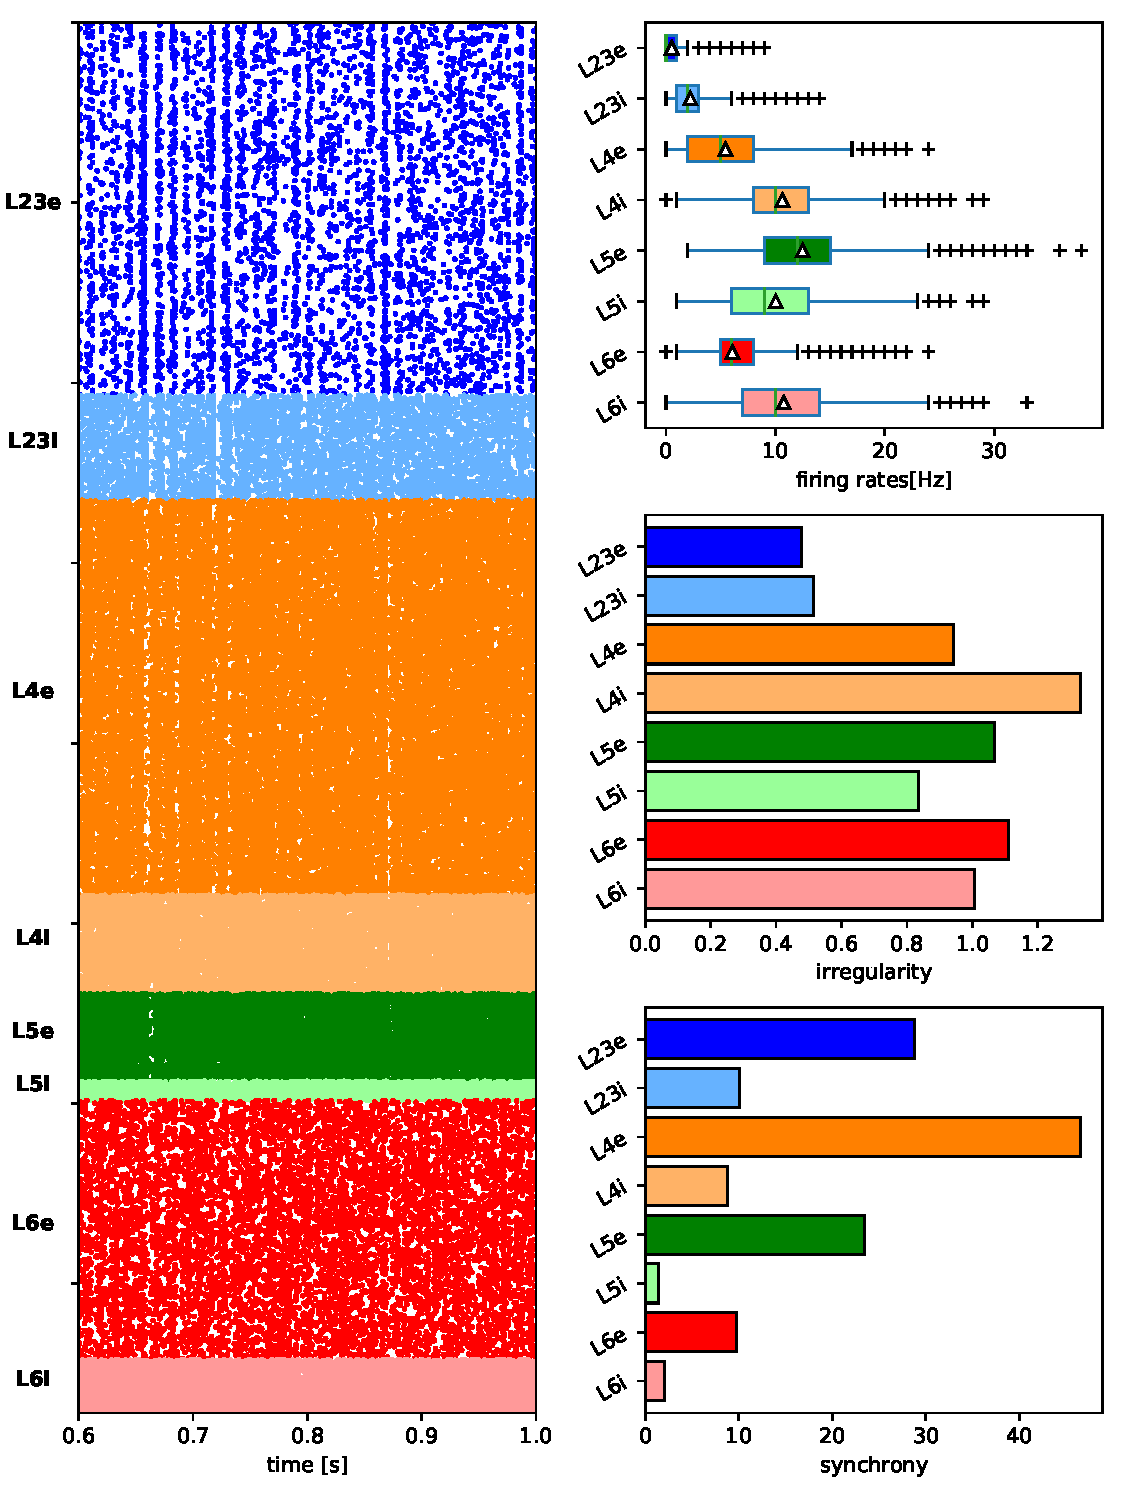
\includegraphics[width=.9\linewidth]{./figures/dGLPD_delta_d1_1s.pdf}
\caption[\textbf{Bottom right:}]{\label{fig:org46f253a}Measures obtained from 1 sec of simulation (\(dt=1\) ms). The first 100 ms was discarded due to its transient bvehavihour. Dark colors indicate excitatory population, and light colors indicate inhibitory population. \textbf{Left:} raster plot of the last 400 ms. \textbf{Top right:} mean firing rate per cortical layer. \textbf{Center right:} Irregularity measured as the coefficient of variation (CV) of the interspike interval (ISI). \textbf{Bottom right:} The synchrony index is computed as the variance of the spike count histogram divided by its mean.}
\end{figure}


\subsubsection{Simulation time step of 0.1 ms}
\label{sec:org6949eb6}

\begin{minted}[bgcolor=shadecolor,fontsize=\scriptsize]{sh}
time ./dGLPD_delta 11111 1000 0.1
\end{minted}

\begin{minted}[bgcolor=shadecolor,fontsize=\scriptsize]{text}
Random Number Generator Engine: xoroshiro128+
seed: 11111, Simulation time: 1000 ms, Simulation time step: 0.1 ms
prepare: 362.266 s
simulate(1000): 269.677 s

real    10m32.913s
user    10m11.589s
sys     0m20.644s
\end{minted}

\begin{figure}[htbp]
\centering
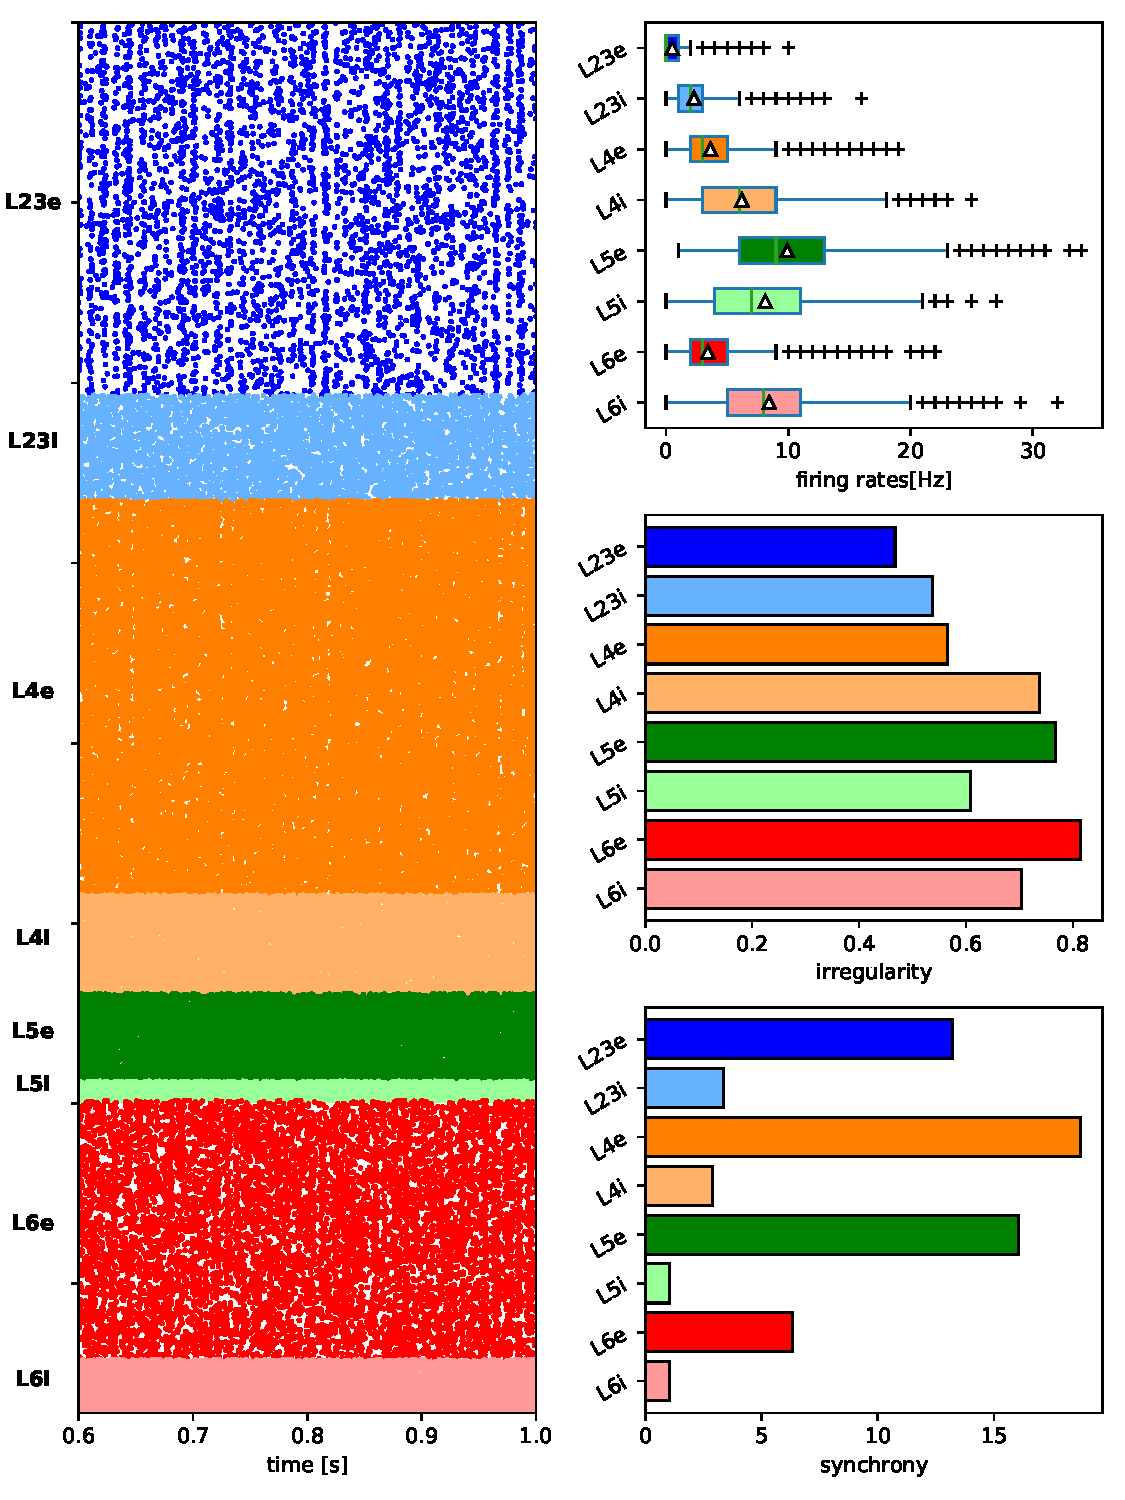
\includegraphics[width=.9\linewidth]{./figures/dGLPD_delta_d01_1s.pdf}
\caption[\textbf{Bottom right:}]{\label{fig:org5da79d9}Measures obtained from 1 sec of simulation (\(dt=0.1\) ms). The first 100 ms was discarded due to its transient bvehavihour. Dark colors indicate excitatory population, and light colors indicate inhibitory population. \textbf{Left:} raster plot of the last 400 ms. \textbf{Top right:} mean firing rate per cortical layer. \textbf{Center right:} Irregularity measured as the coefficient of variation (CV) of the interspike interval (ISI). \textbf{Bottom right:} The synchrony index is computed as the variance of the spike count histogram divided by its mean.}
\end{figure}


\subsubsection{NEST 2.16, simulation time step 0.1 ms}
\label{sec:orga82b34c}

\begin{minted}[bgcolor=shadecolor,fontsize=\scriptsize]{sh}
module load py36-nest/2.16.0
time python3 example.py
\end{minted}

\begin{minted}[bgcolor=shadecolor,fontsize=\scriptsize]{text}
Spike detectors created
Thalamic input not provided
Poisson background input created
Recurrent connections are established
Poisson background input is connected
Spike detector connected
Time to create the connections: 224.70 s

May 04 09:26:07 NodeManager::prepare_nodes [Info]: 
    Preparing 77185 nodes for simulation.

May 04 09:27:13 SimulationManager::start_updating_ [Info]: 
    Number of local nodes: 77185
    Simulation time (ms): 1000
    Number of OpenMP threads: 1
    Number of MPI processes: 1

100 %: network time: 1000.0 ms, realtime factor: 0.0002 

May 04 11:13:29 SimulationManager::resume [Info]: 
    Simulation finished.
Time to simulate: 6442.45 s

real	111m18.500s
user	107m4.390s
sys	3m33.969s
\end{minted}

\subsubsection{NEST 2.20.1, simulation time step 0.1 ms}
\label{sec:org724c0ce}

\begin{minted}[bgcolor=shadecolor,fontsize=\scriptsize]{sh}
module load py36-nest/2.20.1
time python3 example.py
\end{minted}

\begin{minted}[bgcolor=shadecolor,fontsize=\scriptsize]{text}
Spike detectors created
Thalamic input not provided
Poisson background input created
Recurrent connections are established
Poisson background input is connected
Spike detector connected
Time to create the connections: 58.93 s

May 04 09:14:18 NodeManager::prepare_nodes [Info]: 
    Preparing 77233 nodes for simulation.

May 04 09:14:43 SimulationManager::start_updating_ [Info]: 
    Number of local nodes: 77233
    Simulation time (ms): 1000
    Number of OpenMP threads: 4
    Number of MPI processes: 1

100 %: network time: 1000.0 ms, realtime factor: 0.0109

May 04 09:16:17 SimulationManager::run [Info]: 
    Simulation finished.
Time to simulate: 119.92 s

real	3m2.829s
user	10m21.236s
sys	0m32.026s
\end{minted}

\subsection{Memory usage}
\label{sec:org1e9b356}

For measuring memory usage, the code was compiled without optimization (-O0) with debug code (-g), and profiled with valgrind.

\subsubsection{Simulation time step of 1.0 ms}
\label{sec:orgc55b945}

\begin{minted}[bgcolor=shadecolor,fontsize=\scriptsize]{sh}
cmake -DCMAKE_CXX_FLAGS=-g -Dwith-optimize=-O0 ../src
make
valgrind --tool=massif ./dGLPD_delta 1111 1000 1.0
ms_print ./massif.out.18029
\end{minted}

\begin{minted}[bgcolor=shadecolor,fontsize=\scriptsize]{text}
--------------------------------------------------------------------------------
Command:            ./dGLPD_delta 12345 1000 1.0
Massif arguments:   (none)
ms_print arguments: ./massif.out.18029
--------------------------------------------------------------------------------


    GB
13.67^                                                                       :
     |                                                        @:@@###########:
     |                                                        @ @@#          :
     |                                                    @@::@ @@#          :
     |                                                 :@@@@ :@ @@#          :
     |                                            ::::::@@@@ :@ @@#          :
     |                                         ::::  :::@@@@ :@ @@#          :
     |                                  :::::::: ::  :::@@@@ :@ @@#          :
     |                                 @:    ::: ::  :::@@@@ :@ @@#          :
     |                             @@@@@:    ::: ::  :::@@@@ :@ @@#          :
     |                          :@:@@  @:    ::: ::  :::@@@@ :@ @@#          :
     |                       ::::@ @@  @:    ::: ::  :::@@@@ :@ @@#          :
     |                   ::::: ::@ @@  @:    ::: ::  :::@@@@ :@ @@#          :
     |                @:@::: : ::@ @@  @:    ::: ::  :::@@@@ :@ @@#          :
     |                @:@::: : ::@ @@  @:    ::: ::  :::@@@@ :@ @@#          :
     |                @:@::: : ::@ @@  @:    ::: ::  :::@@@@ :@ @@#          :
     |                @:@::: : ::@ @@  @:    ::: ::  :::@@@@ :@ @@#          :
     |         :::::::@:@::: : ::@ @@  @:    ::: ::  :::@@@@ :@ @@#          :
     |        @:     :@:@::: : ::@ @@  @:    ::: ::  :::@@@@ :@ @@#          :
     |  :@@:::@:     :@:@::: : ::@ @@  @:    ::: ::  :::@@@@ :@ @@#          :
   0 +----------------------------------------------------------------------->Ti
     0                                                                   2.649

\end{minted}

\subsubsection{Simulation time step of 0.1 ms}
\label{sec:orgeb40b36}

\begin{minted}[bgcolor=shadecolor,fontsize=\scriptsize]{sh}
cmake -DCMAKE_CXX_FLAGS=-g -Dwith-optimize=-O0 ../src
make
valgrind --tool=massif ./dGLPD_delta 12345 1000 0.1
ms_print ./massif.out.30417
\end{minted}

\begin{minted}[bgcolor=shadecolor,fontsize=\scriptsize]{text}
--------------------------------------------------------------------------------
Command:            ./dGLPD_delta 12345 1000 0.1
Massif arguments:   (none)
ms_print arguments: ./massif.out.30417
--------------------------------------------------------------------------------


    GB
13.73^                                                                       :
     |                               :@@#####################################:
     |                               @@@#                                    :
     |                             ::@@@#                                    :
     |                           :@::@@@#                                    :
     |                        ::::@::@@@#                                    :
     |                       :: ::@::@@@#                                    :
     |                   :::::: ::@::@@@#                                    :
     |                   @  ::: ::@::@@@#                                    :
     |                :::@  ::: ::@::@@@#                                    :
     |               :: :@  ::: ::@::@@@#                                    :
     |             :::: :@  ::: ::@::@@@#                                    :
     |            ::::: :@  ::: ::@::@@@#                                    :
     |          @:::::: :@  ::: ::@::@@@#                                    :
     |          @:::::: :@  ::: ::@::@@@#                                    :
     |         @@:::::: :@  ::: ::@::@@@#                                    :
     |         @@:::::: :@  ::: ::@::@@@#                                    :
     |    @::::@@:::::: :@  ::: ::@::@@@#                                    :
     |    @:  :@@:::::: :@  ::: ::@::@@@#                                    :
     | :::@:  :@@:::::: :@  ::: ::@::@@@#                                    :
   0 +----------------------------------------------------------------------->Ti
     0                                                                   4.535
\end{minted}

\subsection{Comparison with the original (NEST) implementation}
\label{sec:org3e4f162}

The measures shown in figs. \ref{fig:org46f253a} and \ref{fig:org5da79d9} was obtained from 1s of simulation data. On the other hand, the measures on Fig. 6 of the original work \cite{PotjansDiesmann2014} (fig. \ref{fig:measure_NEST_org}) is based on simulation data of 60 s. For a direct comparison, 60 s. was simulated for both conditions (\(dt=1\) and \(0.1\) ms). Fig. \ref{fig:measure_NEST} shows a re-simulation of the NEST code. Please note that synchrony is about 10 folds different to that of the orinal paper (fig. \ref{fig:measure_NEST_org}), and I am working on to find out the reason. In addition, the synchrony using the implemented GLPD model (figs. \ref{fig:measure_GLPD_1} and \ref{fig:measure_GLPD_01}) was qualitatively similar to that of fig. \ref{fig:measure_NEST}, and may have quantitatively differed due to the slightly different synaptic dynamics (the original NEST implementation uses exponentially dacaying synaptic current, whereas GLPD uses delta synapses).


\subsubsection{Simulation time step of 1 ms}
\label{sec:orge4e45b4}

\begin{minted}[bgcolor=shadecolor,fontsize=\scriptsize]{sh}
time ./dGLPD_delta 98765 60000 1.0
\end{minted}

\begin{minted}[bgcolor=shadecolor,fontsize=\scriptsize]{text}
Random Number Generator Engine: xoroshiro128+
seed: 98765, Simulation time: 60000 ms, Simulation time step: 1 ms
prepare: 370.132 s
simulate(60000): 12721.2 s

real	55m39.426s
user	52m58.152s
sys	1m4.037s
\end{minted}


\subsubsection{Simulation time step of 0.1 ms}
\label{sec:org4c8c143}

\begin{minted}[bgcolor=shadecolor,fontsize=\scriptsize]{sh}
time ./dGLPD_delta 98765 60000 0.1
\end{minted}

\begin{minted}[bgcolor=shadecolor,fontsize=\scriptsize]{text}
Random Number Generator Engine: xoroshiro128+
seed: 98765, Simulation time: 60000 ms, Simulation time step: 0.1 ms
prepare: 367.555 s
simulate(60000): 12721.2 s

real	218m9.308s
user	214m54.626s
sys	2m59.228s
\end{minted}


\begin{figure}
  \subfloat[NEST paper]{
    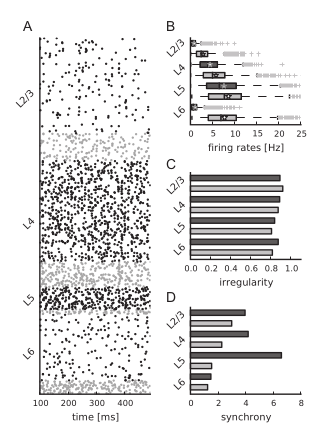
\includegraphics[width=0.5\linewidth]{figures/PD_original_Fig6.png}
    \label{fig:measure_NEST_org}
  }
  \subfloat[NEST sim]{
    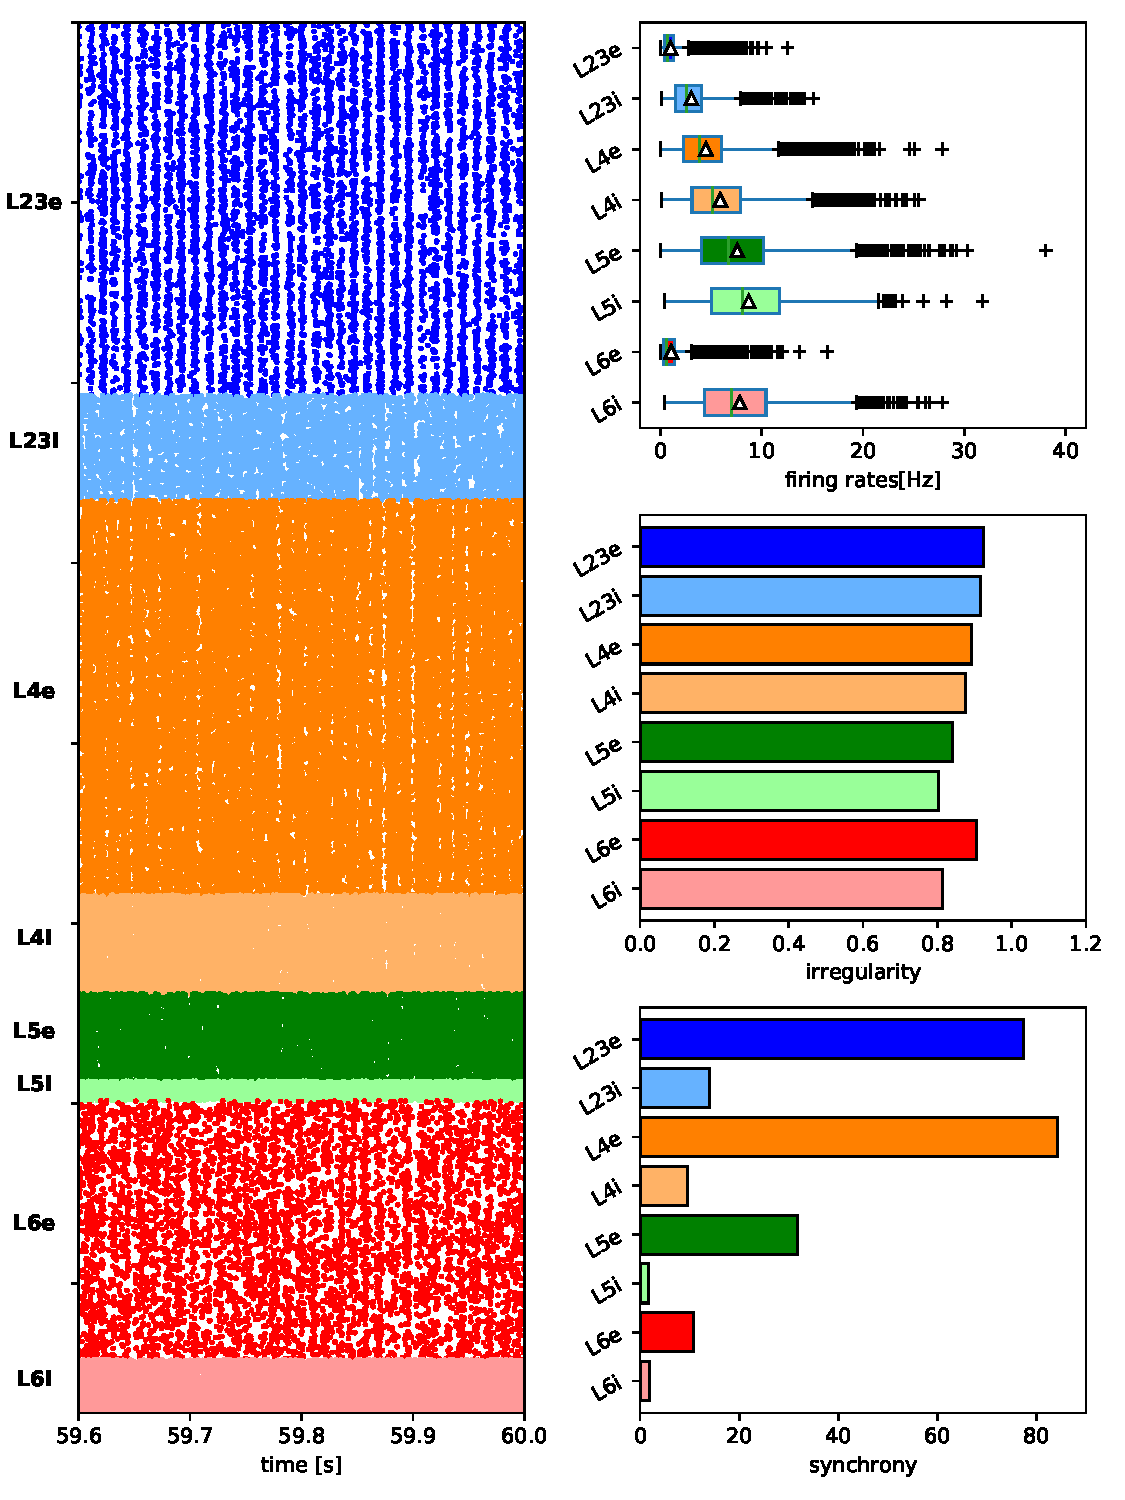
\includegraphics[width=0.5\linewidth]{figures/PD_nest.pdf}
    \label{fig:measure_NEST}
  }
  \newline
  \subfloat[$dt=1$ ms]{
    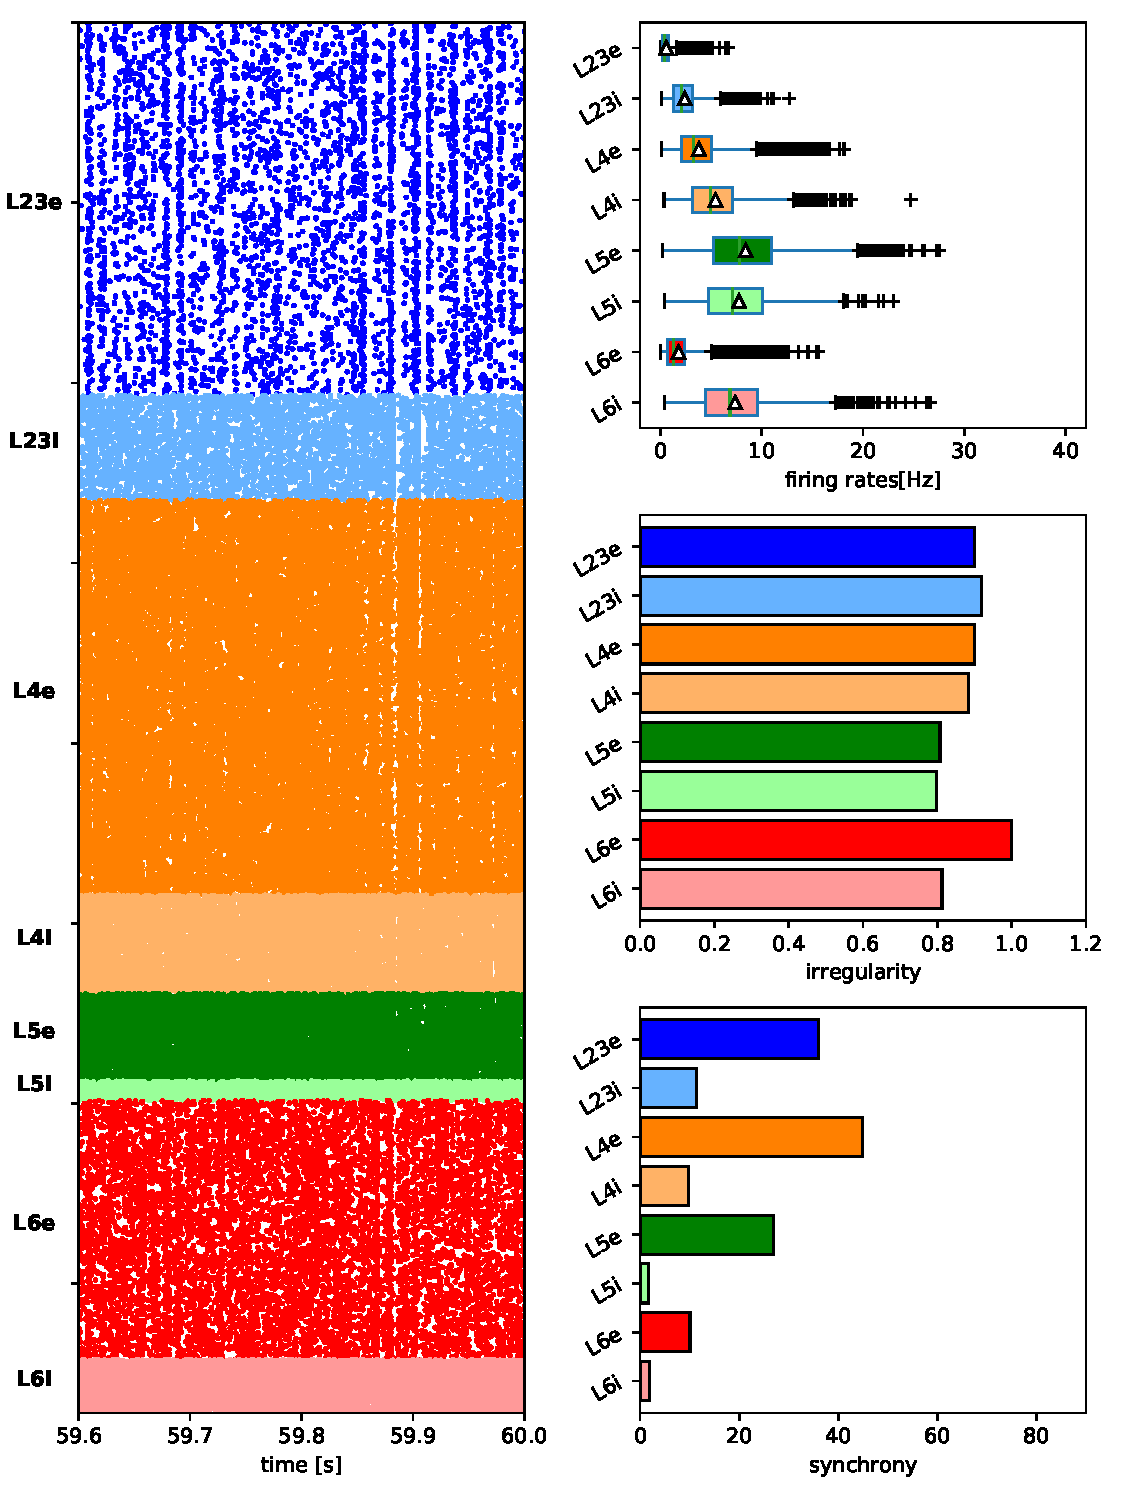
\includegraphics[width=0.5\linewidth]{figures/dGLPD_delta_1.pdf}
    \label{fig:measure_GLPD_1}
  }
  \subfloat[$dt=0.1$ ms]{
    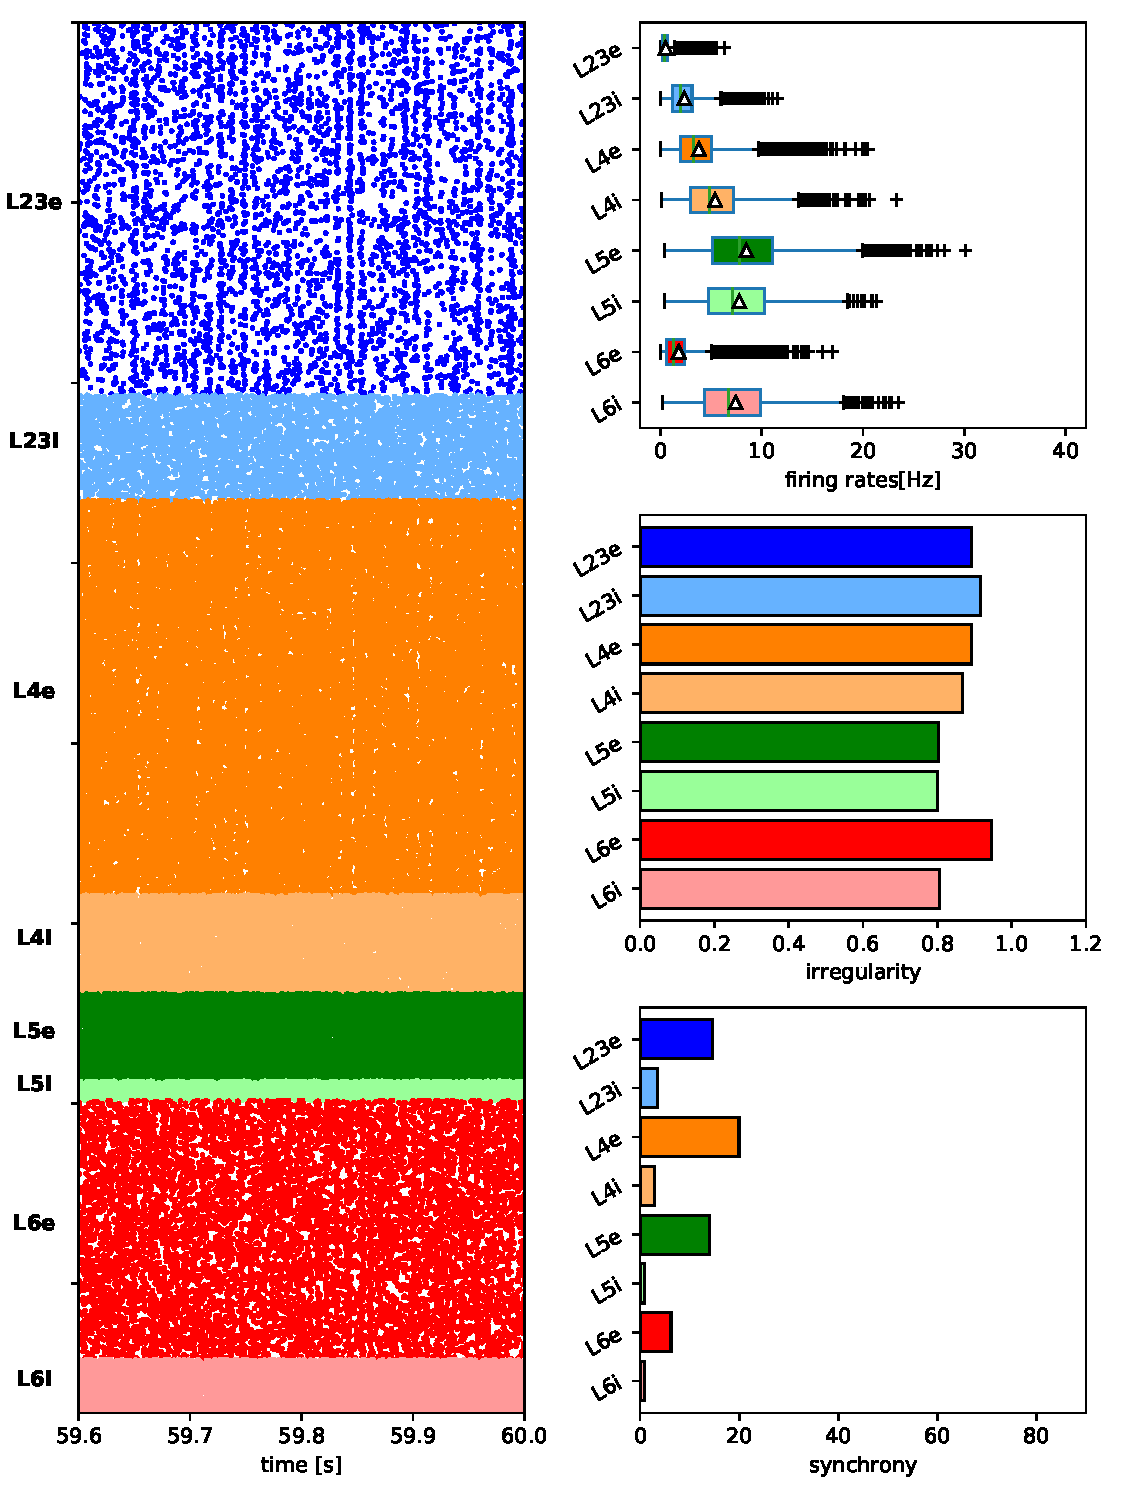
\includegraphics[width=0.5\linewidth]{figures/dGLPD_delta_01.pdf}
    \label{fig:measure_GLPD_01}
  }
    \caption{Measures obtained from 60 sec of simulation ($dt=0.1$ ms). Dark colors indicate excitatory population, and light colors indicate inhibitory population. \textbf{Left:} raster plot of the last 400 ms. \textbf{Top right:} mean firing rate per cortical layer. \textbf{Center right:} Irregularity measured as the coefficient of variation (CV) of the interspike interval (ISI). \textbf{Bottom right:} The synchrony index is computed as the variance of the spike count histogram divided by its mean.}
    \label{fig:measure_60}
\end{figure}


\subsection{Storage of \(V_m\) every 1.0 ms}
\label{sec:orgeefd06f}

By changing the last argument in line 81 of \texttt{./src/main\_dGLPD\_delta.cpp}, one can enable storage analog data such as \(V_t(i)\) of every neuron at every 1.0 ms interval. In such case, the simulation time for \(dt=0.1\) and \(dt=1.0\) are both about 15 min. This is expected as writing data to file is a time-consuming process.

\subsection{{\bfseries\sffamily TODO} List of future tasks}
\label{sec:org0071579}

\begin{itemize}
\item cross-correlogram
\item effect of considering the delay by a fixed delay of 1 time step for simulations with 1ms time step.
\end{itemize}

\bibliography{local}
\end{document}
